% vim:set spell tw=79:

\documentclass[article]{uibk}
\title{Exploitation Techniques and Mitigations}
\author{Alex Hirsch \and Patrick Ober}
\date{2016-01-31}

\newminted{nasm}{fontsize=\scriptsize,frame=leftline,framesep=2mm,linenos}

\begin{document}

% \maketitle
%
% \section*{Abstract}
% \label{sec:abstract}
%
% \setcounter{tocdepth}{1}
% \tableofcontents
%
% \newpage

\section*{Acknowledgement}

A university course at Rensselaer Polytechnic
Institut\footnote{\url{http://rpi.edu/}} held in Spring 2015 focused on
\textit{Modern Binary Exploitation}. They made their course material available
on GitHub \cite{RPISEC} under the Creative Commons Attribution-NonCommercial
4.0 International
license\footnote{\url{https://creativecommons.org/licenses/by-nc/4.0/legalcode}}.
We reused a lot of their material in this project.

We highly recommend checking them out and having a look at their material for
further details.

\section{Introduction}

Exploiting binaries was comparatively easy in the early days of computing.
Usually there were no special mitigation techniques in place trying to prevent
even the most simplest exploits. This is the point in time where we will start
of. First we talk about two very simple exploits, namely the Format String
Exploit and the Buffer Overflow in combination with Shell Code. Note that there
is a huge collection of exploitation techniques known to the public and we will
thereby only look at a very small fraction of them.

But before we can introduce these two exploits, some background knowledge is
required. This will be handled by the next section, which provides a short
overview of the relevant components in our target architecture, the x86
platform.

After that both techniques are introduced to the reader, followed by the first
mitigation technique, Data Execution Prevention (DEP). From there on we will
keep on using the buffer overflow technique with some adaptations to circumvent
DEP. At this point Return Oriented Programming (ROP) is introduced.

This directly leads to Address Space Layout Randomization (ASLR) the next
mitigation mechanism we will discuss. Again the buffer overflow technique can
be adapted to break ASLR through the use of additional information.

Since neither DEP nor ASLR provide significant protection against even this
simple technique, an additional mitigation is put into place in the form of
Stack Cookies.

Examples will be provided along the way to support the reader and provide some
additional explanation.

Control Flow Integrity (CFI), Heap Corruption and polymorphic code will follow
in a more compressed manner to communicate the main idea behind each of them.

Finally we will conclude with a word about other architectures (x86\_64 and
ARM) and a lookout that even languages considered secure have their own set of
exploitation techniques an attacker could leverage.

\subsection{Main Assumption}

Throughout this work we assume that we know the target binary (and the
libraries it uses). Let us show that this assumption is quite reasonable to
make by looking through the eyes of the adversary. An attacker who wants to
penetrate a target machine and get control over it would most likely choose the
easiest path, by exploiting the weakest link. Most machines relevant to an
attackers interest will run provide multiple services. For example, while the
main server of a small business company may run a homemade communication server
for interaction between them and their clients, it may also run a standard web
server. Sending a misspelled request to the server may lead following response:

\begin{pre*}{autogobble,xleftmargin=1cm}
    <!DOCTYPE HTML PUBLIC "-//IETF//DTD HTML 2.0//EN">
    <html><head>
    <title>400 Bad Request</title>
    </head><body>
    <h1>Bad Request</h1>
    <p>Your browser sent a request that this server could not understand.<br />
    </p>
    <hr>
    <address>Apache/2.2.22 (Ubuntu) Server at ovinnik.canonical.com Port 80</address>
    </body></html>
    Connection closed by foreign host.
\end{pre*}

The web server tells us his exact version and since it also provides
information about the operating system an attacker can easily copy the basic
setup to test and tweak his exploits.

\section{Platform x86}

This section will teach necessary background knowledge about the target
platform to fully conceive the following techniques. But first let us elaborate
why x86 has been chosen in the first place.

At the time these techniques (and the related mitigations) were established,
x86 was the most common platform. Since most exploits easily translate over
from x86 to other architectures, especially x86\_64 which very common nowadays.
Also, most material found on the internet regarding this and related topics
cover x86.

More detailed explanations can be found on
Wikipedia\footnote{\url{https://en.wikipedia.org/wiki/X86}} or the Intel
Manual\footnote{\url{https://www-ssl.intel.com/content/www/us/en/processors/architectures-software-developer-manuals.html}}.

\subsection{CPU and registers}

\begin{figure}[htpb]
    \centering
    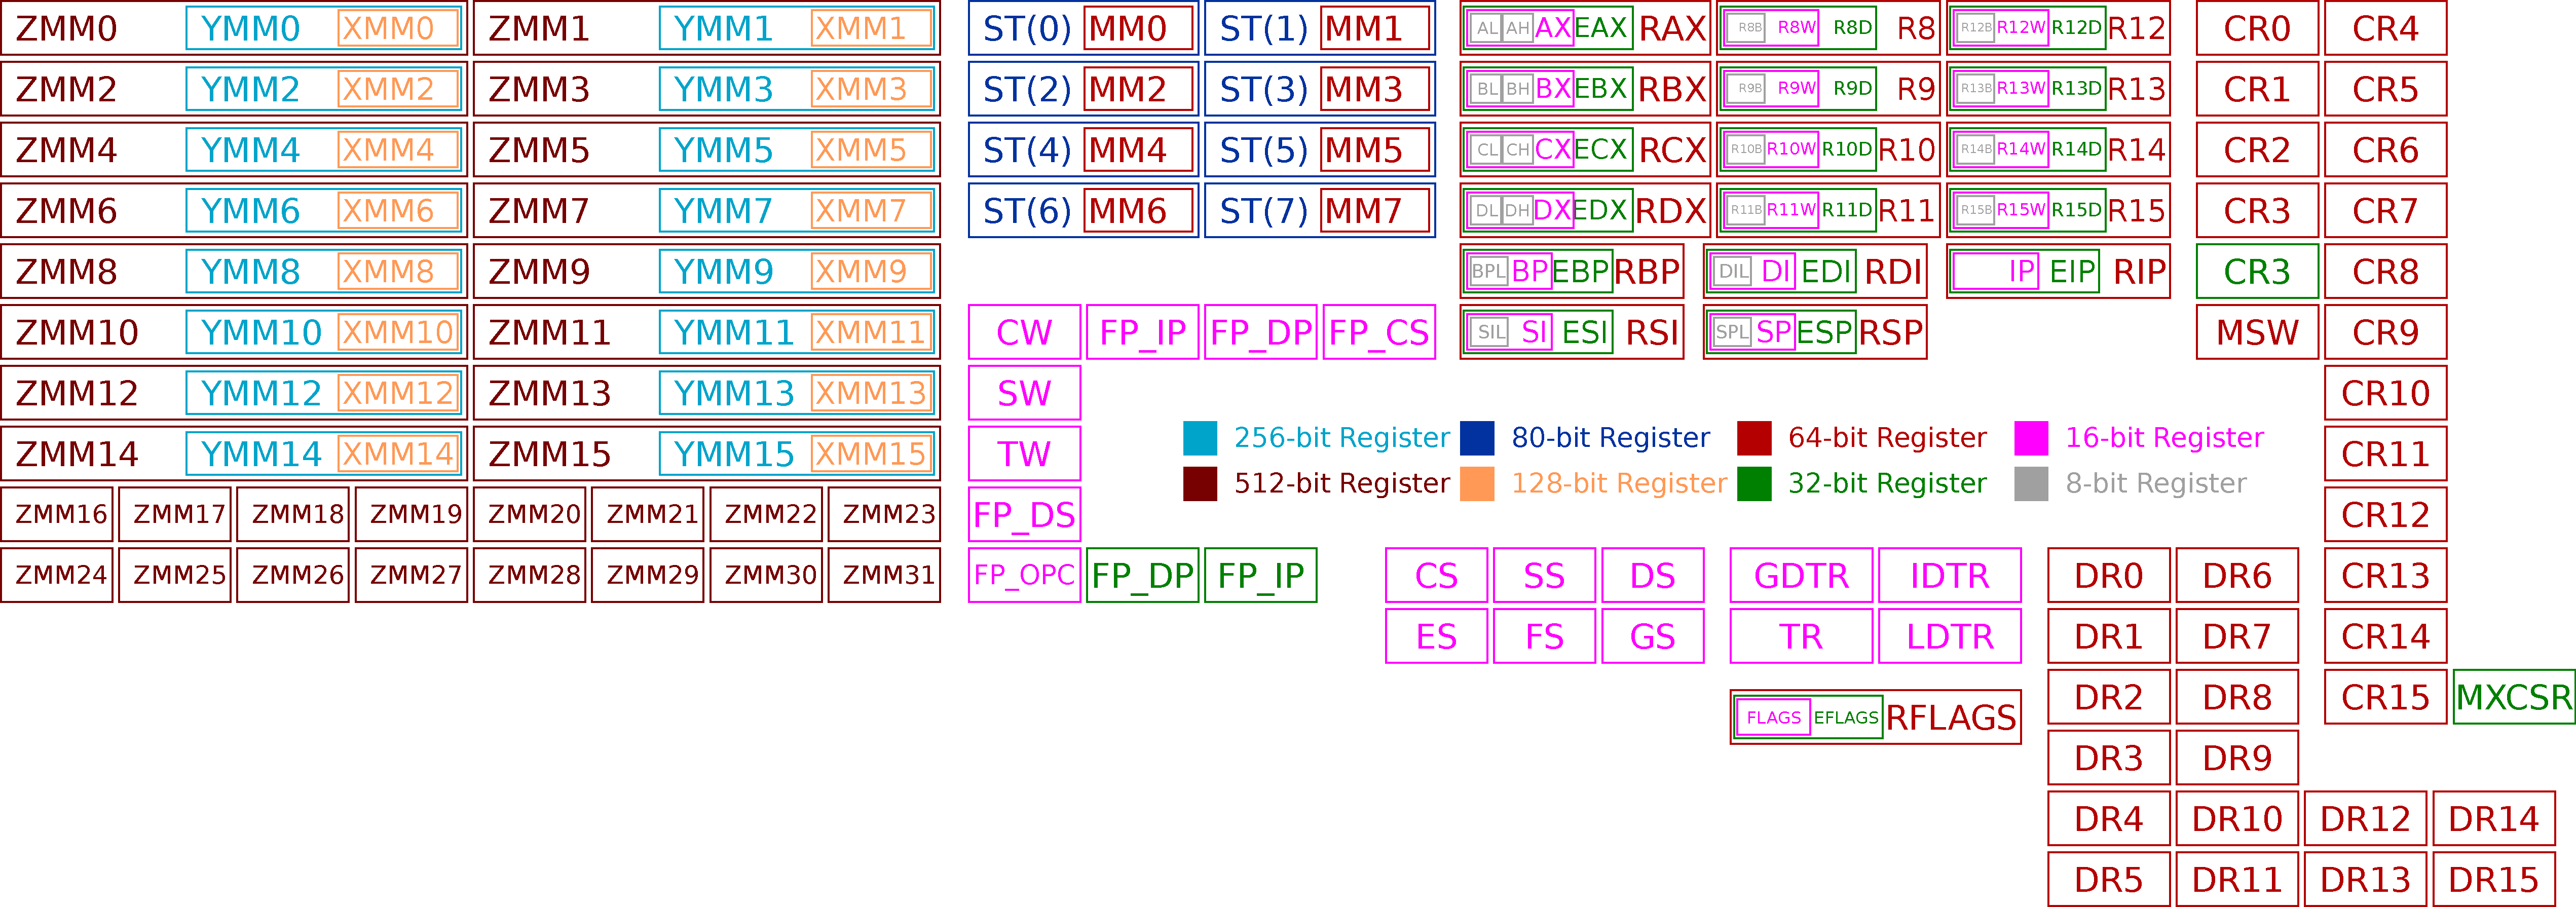
\includegraphics[width=\textwidth]{gfx/x86_registers.pdf}
    \caption{Register overview including \SI{64}{\bit} extension}
    \label{fig:registers}
\end{figure}

\Cref{fig:registers} (from
Wikipedia\footnote{\url{https://en.wikipedia.org/w/index.php?title=X86&oldid=696308590\#/media/File:Table_of_x86_Registers_svg.svg}})
shows an overview of registers available on the x86 platform. While there are
dedicated registers for floating pointer operations and also special registers
which hardware protection (segment registers) we will only focus on nine most
commonly used registers.

\begin{minipage}[t]{0.5\textwidth}
    \begin{description}
        \item[\texttt{EAX}] Accumulator Register
        \item[\texttt{EBX}] Base Register
        \item[\texttt{ECX}] Counter Register
        \item[\texttt{EDX}] Data Register
        \item[\texttt{ESI}] Source Index
        \item[\texttt{EDI}] Destination Index
        \item[\texttt{EBP}] Base Pointer
        \item[\texttt{ESP}] Stack Pointer
        \item[\texttt{EIP}] Instruction Pointer
    \end{description}
\end{minipage}
\begin{minipage}[t]{0.45\textwidth}
    \begin{figure}[H]
        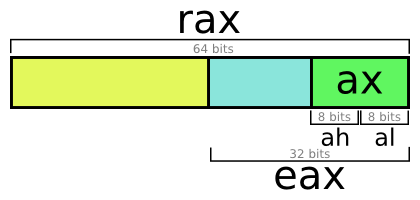
\includegraphics[width=\textwidth]{gfx/single_register.png}
        \caption{Addressing specific parts of a register including \SI{64}{\bit} extension}
        \label{fig:single_register}
    \end{figure}
\end{minipage}
\bigskip

The instruction pointer \texttt{EIP} points to the next instruction located in
memory which is going to be executed on the cycle. Stack pointer \texttt{ESP} and base
pointer \texttt{EBP} are used for stack management which is vital to call and
return from multiple functions properly. The remaining six registers are used
for computation and passing arguments for system calls. Their values can either
be interpreted as integers or pointers.

Note that these registers can be addressed partially allowing one to write only
to the lower \SI{16}{bit} for example as displayed in
\cref{fig:single_register} taken from \textit{null
programm}\footnote{\url{http://nullprogram.com/img/x86/register.png} on
December of 2015}.

The CPU comes with protection mechanisms which allows the operating system
kernel to limit the privileges of other processes. This mechanism is known as
\textit{protection rings} (Ring 0 -- Ring 3). The kernel runs \emph{in} Ring 0
(most privileged) and switches to Ring 3 (least privileged) when a normal
process is scheduled. A system call has to be made by the process if it needs
something which goes beyond its scope. The kernel takes over, deals with the
request and returns execution back to the process. This is known as
\textit{context switch} and switching between Rings happens along the way.

\subsection{System Calls}

As already mentioned in the previous paragraph, a process only has limited
capabilities and the kernel has to take over to fulfill certain (more
privileged) operations. The operating system's documentation tells you which
system calls are available (on which platform) and what additional parameters
they require. Let us illustrate this with an example: On x86 the Linux system
number 4 (starting from 0) is the \texttt{sys\_write} system call which writes
data to a file descriptor. It takes three arguments, the file descriptor to
write to, a pointer to the start of the data which should be written and the
length of the data. The number of the system call together with these three
parameters are placed in the \texttt{EAX}, \texttt{EBX}, \texttt{ECX},
\texttt{EDX} respectively. To invoke the system call issue following
instruction:

\begin{nasmcode*}{autogobble,xleftmargin=1cm,linenos=false}
    int     0x80
\end{nasmcode*}

Nowadays you may encounter a different mechanism for system calls, the Virtual
Dynamic Shared Objects (vDSO) mechanism. This goes beyond our scope here, we
will use the previously mentioned mechanism in our exploits. If interested, you
may want to look at the related man
page\footnote{\url{http://man7.org/linux/man-pages/man7/vdso.7.html}}.

\subsection{Memory}

Physical memory is managed by the operation system kernel by utilising the
Memory Management Unit (MMU). Each process' address space is virtualized and
memory operations are translated on-the-fly by the MMU. The physical memory is
segmented into \textit{pages} (typically \SI{4}{\kibi\byte} in size) and each
page can be mapped into the virtual address space of one or more (shared)
processes.~\cite[pp.~400]{unix_interals}

The main parts located inside the (virtual) address space of a process are the
executable itself with its \texttt{.text} and \texttt{.data} section, the heap
used for dynamic data, the stack used for local variables and function calling
and used libraries.

\subsection{Endianness}
\label{sub:endianness}

\begin{figure}[t]
    \centering
    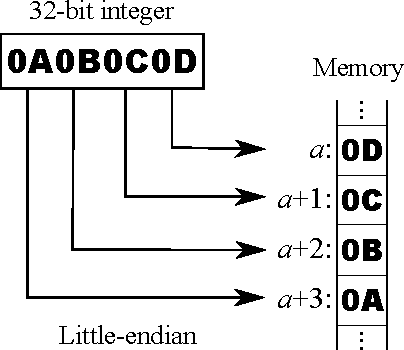
\includegraphics[width=0.35\textwidth]{gfx/little_endian.pdf}
    \caption{Placement of bytes in memory in little-endian}
    \label{fig:little_endian}
\end{figure}

Endianness refers to the byte order used when storing data in memory (or
transmitting it over the network). \Cref{fig:little_endian} (from
Wikipedia\footnote{\url{https://en.wikipedia.org/w/index.php?title=Endianness&oldid=696417697\#/media/File:Little-Endian.svg}})
illustrates that the least significant byte of a word is placed at the lower
memory address and successive bytes are placed as the memory address increases.

\subsection{Calling Convention}
\label{sub:calling_convention}

A calling convention defines how function calls should be implemented. What
calling convention is used depends on the platform, toolchain and (compiler)
settings. Let us exhibit what the convention defines and what convention we are
using.

\begin{minipage}[t]{0.47\textwidth}
    Defines:
    \begin{itemize}
        \item Where to place arguments
        \item Where to place return value
        \item Where to place return address
        \item Who prepares the stack
        \item Who saves which register
        \item Who cleans up\\
            (caller or callee)
    \end{itemize}
\end{minipage}
\begin{minipage}[t]{0.47\textwidth}
    C Declaration (cdecl):
    \begin{itemize}
        \item Arguments on stack (reverse order)\\
            stack aligned to \SI{16}{\byte} boundary
        \item Return via register (\texttt{EAX} / \texttt{ST0})
        \item \texttt{EAX}, \texttt{ECX}, \texttt{EDX} saved by the caller\\
            rest saved by the callee
        \item On stack:\\
            old instruction pointer (\texttt{IP})\\
            old base pointer (\texttt{BP})
        \item Caller does the cleanup
    \end{itemize}
\end{minipage}

\section{Format String Exploits}

The first exploitation technique we will discuss builds upon the interpretation
of format strings. \texttt{printf} is a C function of the standard library
which will interpret such strings and print them to \texttt{stdout}. As the
name already tells you, the supplied string contains \textit{formatter}
describing how to actually handle additional arguments. If you are unfamiliar
with \texttt{printf} please have a look at the man
page\footnote{\url{http://linux.die.net/man/3/printf}}.

Taking a closer look at \texttt{printf} we can see that its first argument is a
format string followed by a variable number of additional arguments. In C you
don't know how many arguments have been supplied when a function with a
variable number of arguments is called. Some instances work around this by
taking an argument count as their first argument, others expect you to
terminate with a special symbol (usually \texttt{NULL}). \texttt{printf} uses
the format string to derive how many arguments have been supplied. Calling
\texttt{printf}, for example, with the string \texttt{"\%d + \%d = \%d"}
assumes that (at least) three arguments have been provided.

\begin{listing}[h!]
    \begin{minipage}[t]{0.47\textwidth}
        \cfile{../format_string/main.c}
    \end{minipage}
    \begin{minipage}[t]{0.47\textwidth}
        \begin{pre*}{autogobble}
            > echo foobar | ./main
            You entered:
            foobar
        \end{pre*}
        \medskip
        \begin{pre*}{autogobble}
            > echo AAAABBBB | ./main
            correct
        \end{pre*}
        \medskip
        \begin{pre*} {autogobble}
            > echo '%08x' | ./main
            You entered:
            bfd98ed4
        \end{pre*}
    \end{minipage}
    \caption{Program vulnerable to Format String Exploits}
    \label{src:format_string_exploit}
\end{listing}

The exploit comes from the notion that a format string provided by an attacker
gets interpreted. The program shown in \cref{src:format_string_exploit} will
take an arbitrary string from \texttt{stdin} and pass it on to \texttt{printf}.
For simple inputs (not containing formatter) this works fine. But as soon as
formatter are provided, \texttt{printf} is going to access the locations where
the corresponding arguments \emph{would} be located. From the calling
convention described in \cref{sub:calling_convention} we know that these
arguments would be located on the stack, therefore \texttt{printf} will print
whatever lies on the stack.

To fully exploit the provided example, note that an attacker in this scenario
wants to get a hold of the hardcoded password stored in \texttt{passwd}. Since
local variables are placed on the stack \texttt{printf} will be able to read
the password if enough formatters are provided:

\begin{pre*} {autogobble}
    > python -c 'print "%08x." * 10' | ./main
    bf920c14.00000064.b77de29e.00000000.00000000.b77fedf8.bf920d94.00000000.41414141.42424242.
\end{pre*}

Here we use Python to craft the format string for us. As we can see the
password is printed (ASCII encoded). Byte order is swapped because of
endianness (see \cref{sub:endianness}). Apart from the password we also gather
a bunch of pointers, these can be used later on to break ASLR (see
\cref{sub:info_leak}).

We would like to point the reader to the book \textit{Hacking: The Art of
Exploitation} \cite[pp.~167]{art_of_exploitation} for more details about this
technique. We will come back to this technique later on to show that
\texttt{printf} enables even more sophisticated attacks.

\newpage

\section{Buffer Overflow}

\section{Shell Code}

\section{Data Execution Prevention (DEP)}

\section{Return Oriented Programming (ROP)}

\section{Address Space Layout Randomization (ASLR)}

\section{Stack Cookies}

\section{Control Flow Integrity (CFI)}

\section{Other Architectures}

\section{Conclusion}

\bibliography{references}

\end{document}
